\section{Solving partial differential equations with Green's functions}

\subsection{Diffusion equation and Fourier transform}
Recall the heat equation, \cref{eq:4.3}, for a conducting wire given by
\begin{align} \label{eq:10.1}
	\pdv{\Theta}{t}\qty(x,t) - D\pdv[2]{\Theta}{x}\qty(x,t) = 0
\end{align}
with initial conditions $\Theta(x,0) = h(x)$ and boundary conditions $\Theta \to 0$ as $x \to \pm \infty$.
Taking the Fourier transform with respect to $x$ using \cref{eq:8.13},
\begin{align*}
	\pdv{t} \widetilde \Theta(k,t) = -D k^2 \widetilde \Theta(k,t)
\end{align*}
Integrating, we find
\begin{align*}
	\widetilde \Theta(k,t) = C e^{-D k^2 t}
\end{align*}
The initial conditions give $\widetilde \Theta(k,0) = \widetilde h(k)$ and therefore
\begin{align*}
	\widetilde \Theta(k,t) = \widetilde h(k) e^{-Dk^2 t}
\end{align*}
We take the inverse Fourier transform to find
\begin{align*}
	\Theta(x,t) = \frac{1}{2\pi} \int_{-\infty}^\infty \widetilde h(k) \underbrace{e^{-Dk^2 t}}_{\mathclap{\text{FT of Gaussian}}} e^{ikx} \dd{k}
\end{align*}
Hence, by the convolution theorem \cref{eq:8.17},
\begin{align} \label{eq:10.2}
	\Theta(x,t) &= \frac{1}{\sqrt{4 \pi D t}} \int_{-\infty}^\infty h(u) \exp(-\frac{(x-u)^2}{4Dt}) \dd{u} \notag \\
	&\equiv \int_{-\infty}^\infty h(u) S_d(x-u,t) \dd{u}
\end{align}
where the \textit{fundamental solution} is
\begin{align} \label{eq:10.3}
	S_d(x,t) = \frac{1}{\sqrt{4 \pi D t}} \exp(-\frac{x^2}{4Dt})
\end{align}
which is the Fourier transform of $\exp(-D k^2 t)$ (you should know how to derive $\cref{eq:10.3}$ using derivatives or by completing the square).
This is also known as the diffusion kernel or the source function.
\begin{note}
	With localised initial conditions $\Theta(x,0) = \Theta_0 \delta(x)$, the solution is exactly the fundamental solution:
	\begin{align} \label{eq:10.4}
		\Theta(x,t) = \Theta_0 S_d(x,t) = \frac{\Theta_0}{\sqrt{4 \pi D t}} \exp(-\eta^2);\quad \eta = \frac{x}{2\sqrt{Dt}}
	\end{align}
	where $\eta$ is the similarity parameter.
	I.e. for $t \geq 0$ spreads smoothly as a Gaussian.
\end{note} 

\subsection{Gaussian pulse for heat equation}
Suppose that the initial conditions for the heat equation are given by
\begin{align*}
	f(x) = \sqrt{\frac{a}{\pi}} \Theta_0 e^{-ax^2}
\end{align*}
Then, our \cref{eq:10.2} gives
\begin{align*}
	\Theta(x,t) &= \frac{\Theta_0 \sqrt{a}}{\sqrt{4 \pi^2 D t}} \int_{-\infty}^\infty \exp[-au^2 - \frac{(x-u)^2}{4 D t}] \dd{u} \\
    &= \frac{\Theta_0 \sqrt{a}}{\sqrt{4 \pi^2 D t}} \int_{-\infty}^\infty \exp[-\frac{(1 + 4 a D t)u^2 - 2xu + x^2}{4 D t}] \dd{u} \\
    &= \frac{\Theta_0 \sqrt{a}}{\sqrt{4 \pi^2 D t}} \int_{-\infty}^\infty \exp[-\frac{1 + 4 a D t}{4 D t} \qty(u - \frac{x}{1+4aDt}) ] \exp[ \frac{-ax^2}{1+4aDt}] \dd{u}
\end{align*}
Recall \cref{eq:6.3},
\begin{align*}
	\int_{-\infty}^\infty \exp[\frac{-(u - \mu)^2}{\sigma^2}] \dd{u} = \sigma \sqrt{\pi}
\end{align*}
The integral above is a Gaussian, so its solution can be read off directly as
\begin{align} \label{eq:10.5}
	\Theta(x,t) = \frac{\Theta_0 \sqrt{a}}{\sqrt{\pi (1 + 4 \pi^2 D t)}} \exp[\frac{-ax^2}{1+4aDt}]
\end{align}
So the width of the Gaussian pulse will get wider over time, according to $\sigma^2 \sim t$, as it evolves according to the heat equation.
The area is constant, so heat energy is conserved in the system.

\subsection{Forced diffusion equation}
Consider the equation
\begin{align} \label{eq:10.6}
	\pdv{t}\Theta(x,t) - D \pdv[2]{\Theta}{x}(x,t) = f(x,t)
\end{align}
subject to homogeneous initial conditions $\Theta(x,0) = 0$.
We construct a two-dimensional Green's function $G(x,t; \xi, \tau)$ such that
\begin{align} \label{eq:10.7}
	\pdv{t}G(x,t) - D \pdv[2]{G}{x}(x,t) = \delta(x - \xi)\delta(t - \tau)
\end{align}
subject to the same homogeneous boundary conditions $G(x,0;\xi,\tau) = 0$.
Consider the Fourier transform with respect to $x$.
\begin{align*}
	\pdv{\widetilde G}{t} + D k^2 \widetilde G = e^{-ik\xi} \delta(t - \tau)
\end{align*}
We can solve this using an integrating factor $e^{Dk^2 t}$ and integrating with respect to time.
Since $G = 0$ at $t = 0$,
\begin{align*}
	\pdv{t} \qty[ e^{D k^2 t} \widetilde G ] &= e^{-ik\xi + D k^2 t} \delta(t - \tau) \\
	\int_0^t \pdv{t'} \qty[ e^{D k^2 t'} \widetilde G ] \dd{t'} & = \int_0^t e^{-ik\xi + D k^2 t'} \delta(t' - \tau) \dd{t'} \\
	e^{D k^2 t} \widetilde G &= e^{-ik\xi} \int_0^t e^{D k^2 t'} \delta(t' - \tau) \dd{t'} \\
	e^{D k^2 t} \widetilde G &= e^{-ik\xi} e^{D k^2 \tau} H(t - \tau)
\end{align*}
where $H$ is the Heaviside step function.
Thus,
\begin{align*}
	\widetilde G(k,t;\xi,\tau) = e^{-ik\xi} e^{-D k^2 (t - \tau)} H(t - \tau)
\end{align*}
The inverse Fourier transform gives the Green's function.
\begin{align*}
	G(x,t;\xi,\tau) = \frac{H(t - \tau)}{2\pi} \int_{-\infty}^\infty e^{-ik\xi} e^{-D k^2 (t - \tau)} e^{ikx} \dd{k}
\end{align*}
This is a Gaussian; by changing variables into $x' = x - \xi$ and $t' = t - \tau$ we find
\begin{align*}
	G(x,t;\xi,\tau) = \frac{H(t')}{2\pi} \int_{-\infty}^\infty e^{ikx'} e^{-D k^2 t'} \dd{k} = \frac{H(t')}{\sqrt{4 \pi D t'}} \exp[-\frac{(x')^2}{4Dt'}]
\end{align*}
Converting back,
\begin{align} \label{eq:10.8}
	G(x,t;\xi,\tau) = \frac{H(t - \tau)}{\sqrt{4 \pi D (t - \tau)}} \exp[-\frac{(x - \xi)^2}{4D(t - \tau)}] = H(t-\tau) S_d(x-\xi, t-\tau)
\end{align}
where $S_d$ is the fundamental solution in \cref{eq:10.3}.

Thus, the general solution is
\begin{align*}
	\Theta(x,t) = \int_0^\infty \dd{\tau} \int_{-\infty}^\infty \dd{\xi} G(x,t;\xi,\tau) f(\xi, \tau)
\end{align*}
Let $\xi = u$, then
\begin{align} \label{eq:10.9}
	\Theta(x,t) = \int_0^t \dd{\tau} \int_{-\infty}^\infty \dd{u} f(u, \tau) S_d(x-u, t-\tau)
\end{align}

\subsection{Duhamel's principle}
In the above equation, omitting the integral over time, this is exactly the solution as found earlier with initial conditions at $t = \tau$, which was
\begin{align*}
	\Theta(x,t) = \int_{-\infty}^\infty \dd{u} f(u) S_d(x-u, t-\tau)
\end{align*}
The forced PDE with homogeneous boundary conditions can be related to solutions of the homogeneous PDE with inhomogeneous boundary conditions.
The forcing term $f(x,t)$ at $t = \tau$ acts as an initial condition for subsequent evolution.
Thus, the solution, \cref{eq:10.9}, is a superposition of the effects of the initial conditions integrated over $0 < \tau < t$.
This relation between the homogeneous and inhomogeneous problems is known as \textit{Duhamel's principle}.

\subsection{Forced wave equation}
Consider the forced wave equation, given by
\begin{align} \label{eq:10.10}
	\pdv[2]{\phi}{t} - c^2 \pdv[2]{\phi}{x} = f(x,t)
\end{align}
with $\phi(x,0) = \phi_t(x,0) = 0$.
We construct the Green's function using
\begin{align*}
	\pdv[2]{G}{t} - c^2 \pdv[2]{G}{x} = \delta(x-\xi)\delta(t-\tau)
\end{align*}
with $G(x,0) = G_t(x,0) = 0$.
We take the Fourier transform with respect to $x$, and find
\begin{align*}
	\pdv[2]{\widetilde G}{t} + c^2 k^2 \widetilde G = e^{-ik\xi} \delta(t - \tau)
\end{align*}
We can solve this by inspection by comparing with the corresponding initial value problem Green's function \cref{eq:7.26} which has homogeneous solution $\sin kc (t - \tau)$ as $G(x,0) = 0$, and find
\begin{align*}
	\widetilde G = \begin{cases}
		0                                       & t < \tau \\
		e^{-ik\xi} \frac{\sin kc(t - \tau)}{kc} & t > \tau
	\end{cases}
\end{align*}
Using the Heaviside function.
\begin{align*}
	\widetilde G = e^{-ik\xi} \frac{\sin kc(t - \tau)}{kc} H(t - \tau)
\end{align*}
We invert the Fourier transform.
\begin{align*}
	G(x,t;\xi,\tau) = \frac{H(t-\tau)}{2\pi c} \int_{-\infty}^\infty e^{ik(x - \xi)} \frac{\sin kc(t - \tau)}{k} \dd{k}
\end{align*}
Let $A = x - \xi$, and $B = c(t - \tau)$.
By oddness of sine, only the cosine term of the complex exponential remains.
Noting the similarity to the Dirichlet discontinuous function,
\begin{align*}
	G(x,t;\xi,\tau) & = \frac{H(t-\tau)}{\pi c} \int_0^\infty \frac{\cos(kA) \sin(kB)}{k} \dd{k} \\
	& = \frac{H(t-\tau)}{2\pi c} \int_0^\infty \frac{\sin k(A+B) - \sin k(A-B)}{k} \dd{k} \\
	& = \frac{H(t-\tau)}{4c} \qty[ \sgn(A+B) - \sgn(A-B) ]
\end{align*}
by \cref{eq:8.16}.
Since the $H(t - \tau)$ term is nonzero only for $t > \tau$, we must have $B = c(t-\tau) > 0$.
The only way that the bracketed term can be nonzero is when $\abs{A} < B$; so $\abs{x - \xi} < c(t-\tau)$.
This is the domain of dependence as found before, demonstrating the causality of the relation.
Hence,
\begin{align} \label{eq:10.11}
	G(x,t;\xi,\tau) = \frac{1}{2c} H(c(t-\tau) - \abs{x - \xi})
\end{align}
\begin{figure}[h] 
    \centering 
    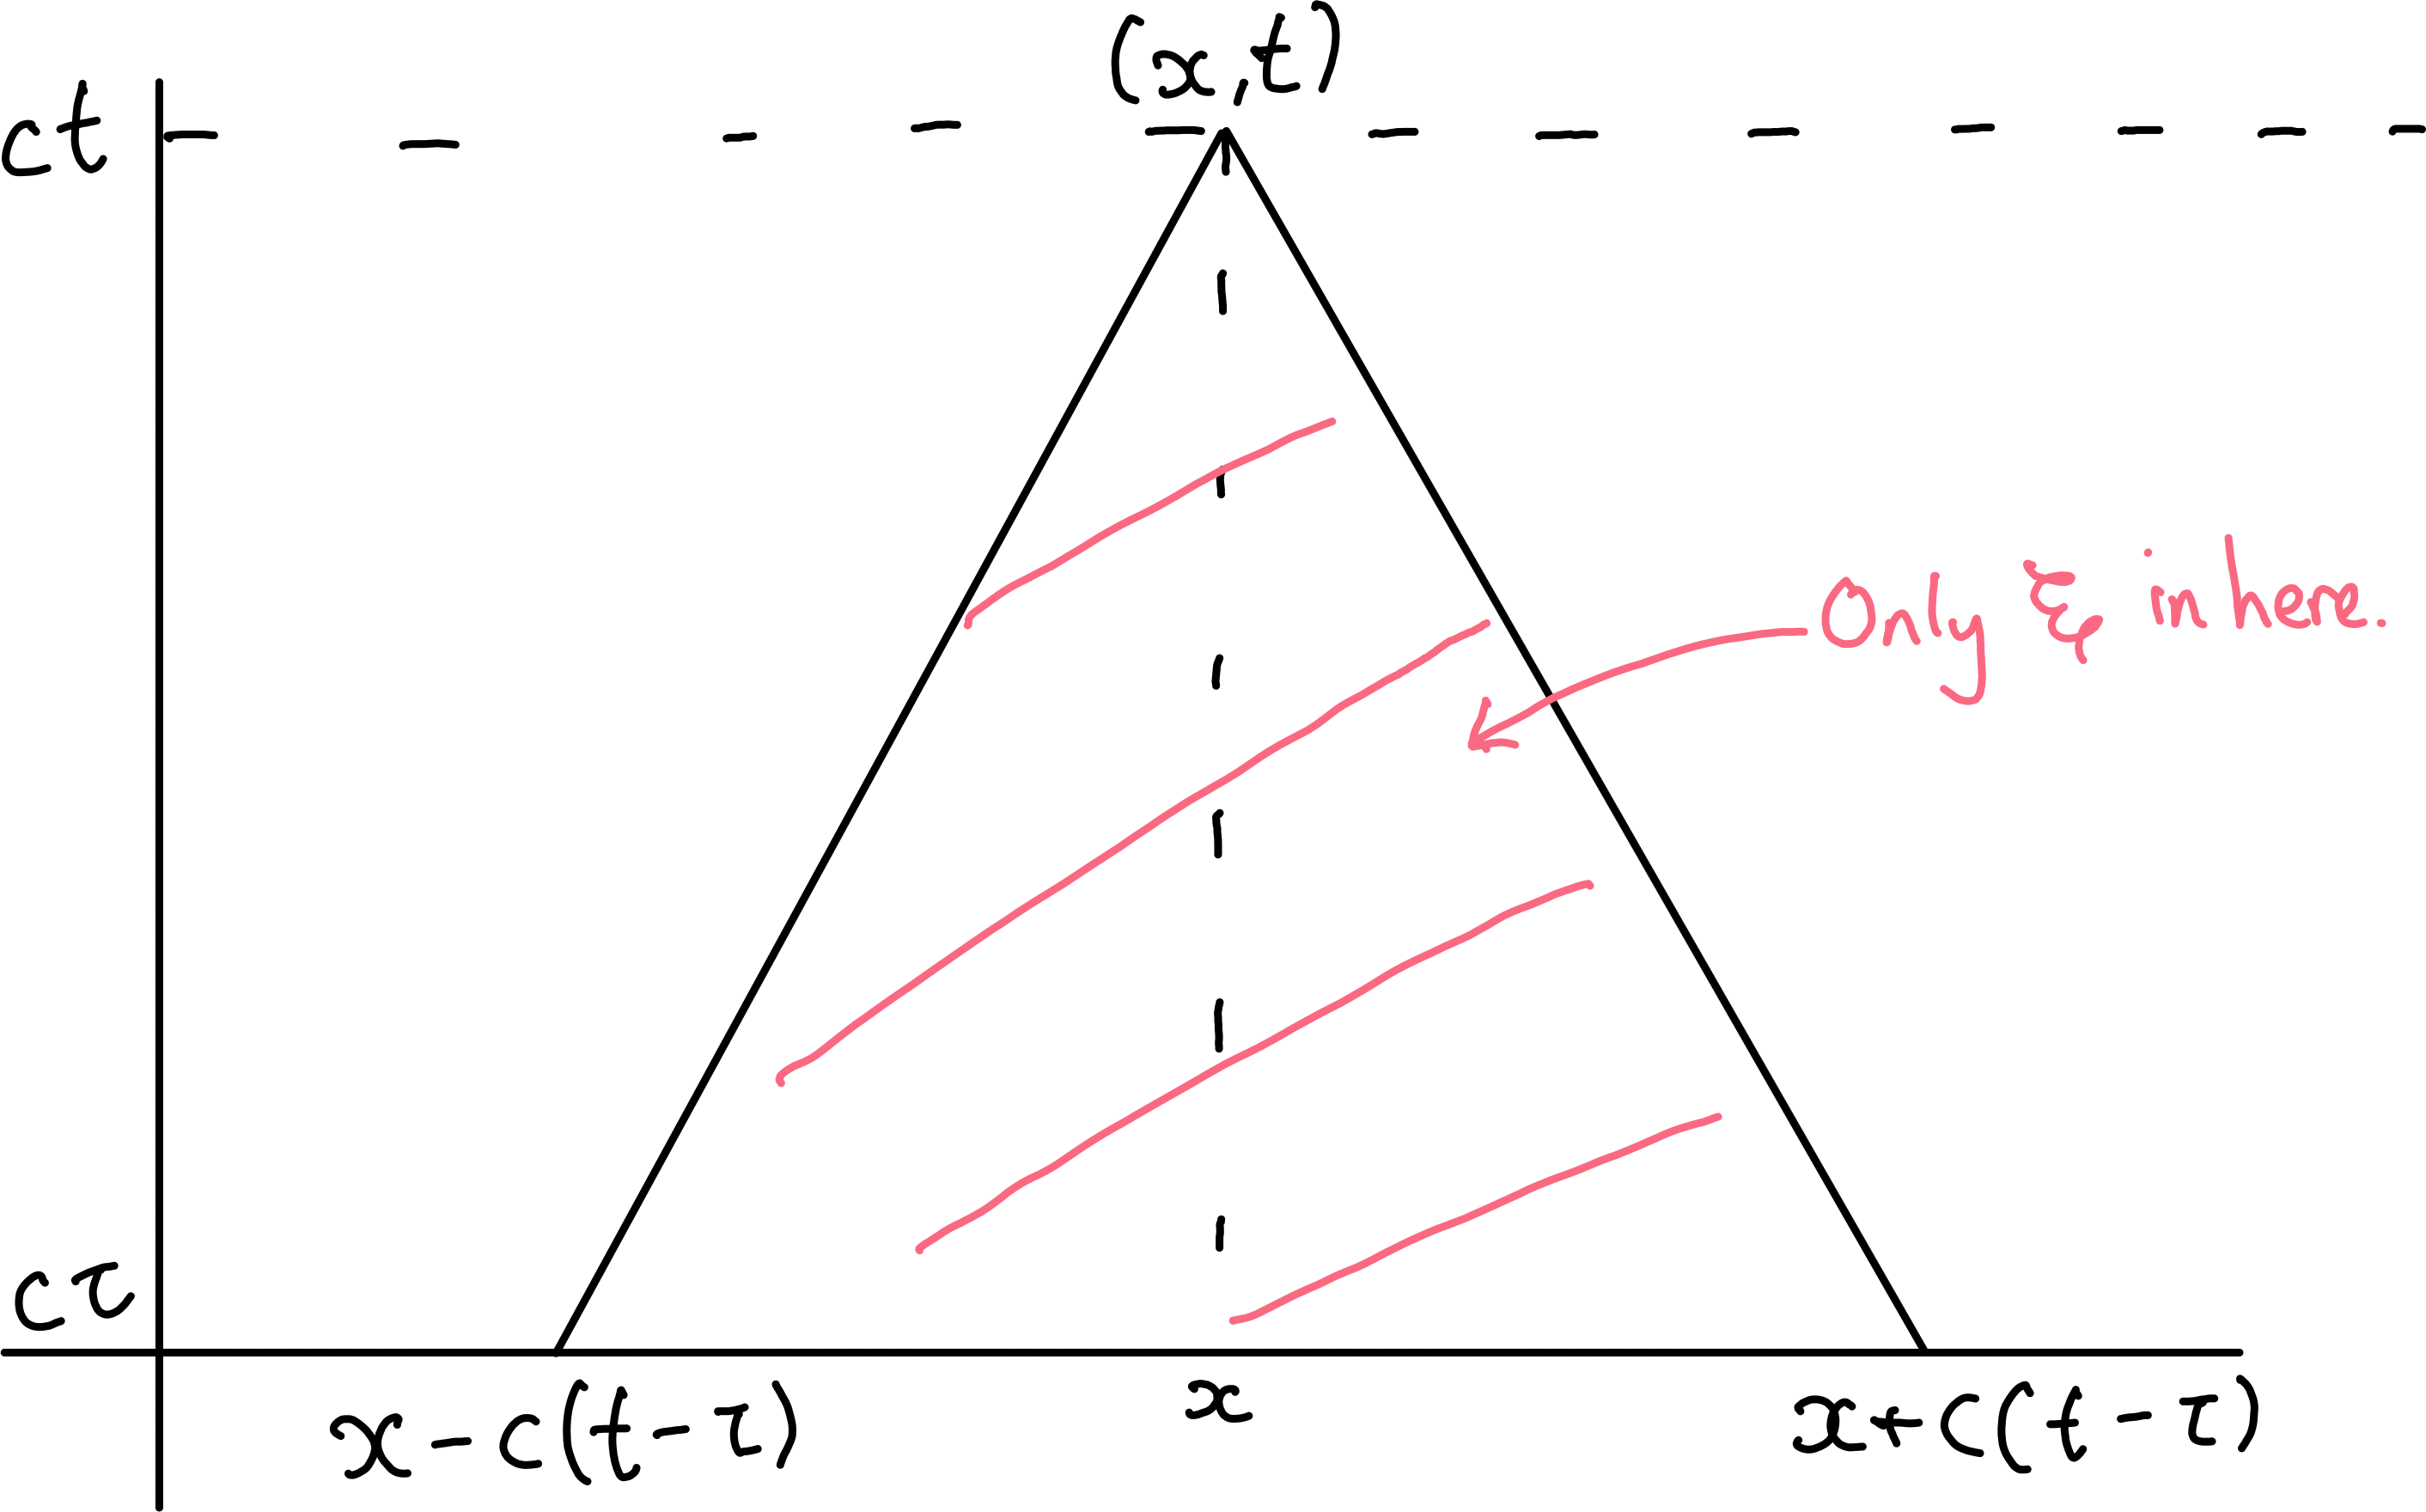
\includegraphics[height=5cm]{10-causality} 
\end{figure}

Thus, the solution is
\begin{align} \label{eq:10.12}
	\phi(x,t) &= \int_0^\infty \dd{\tau} \int_{-\infty}^\infty \dd{\xi} f(\xi, t) G(x,t;\xi,\tau) \notag \\
	&= \frac{1}{2c} \int_0^t \dd{\tau} \int_{x - c(t-\tau)}^{x + c(t - \tau)} \dd{\xi} f(\xi, \tau)
\end{align}

\begin{exercise}
	Relate \cref{eq:10.12} to D'Alembert's solution with ICs \cref{eq:9.18} at $t = 0, \phi = 0, \phi_t = g(x)$ as an example of Duhamel's principle.
\end{exercise} 

\subsection{Poisson's equation}
Consider
\begin{align} \label{eq:10.13}
	\laplacian{\phi} = - \rho(r)
\end{align}
defined on a three-dimensional domain $D$, with Dirichlet boundary conditions $\phi = 0$ on a boundary $\partial D$.

\subsubsection{Fundamental solutions}
The Dirac $\delta$ function, when defined in $\mathbb R^3$, has the following properties.
\begin{enumerate}
	\item $\delta(r - r') = 0$ for all $r \neq r'$;
	\item \begin{align} \label{eq:10.14}
		\begin{cases}
			\int_D \delta(r - r') \dd[3]{r} = 1 & r' \in D \\
			0 & \text{otherwise}
		\end{cases} 
	\end{align} 
	\item $\int_D f(r) \delta(r - r') \dd[3]{r} = f(r')$.
\end{enumerate}
First, we consider $D = \mathbb R^3$ with the homogeneous boundary conditions that $G \to 0$ as $\norm{r} \to \infty$.
This is known as the \textit{free-space} Green's function, denoted $G_{\mathrm{FS}}$,
\begin{align} \label{eq:10.15}
	\laplacian{G_{\mathrm{FS}}}(r, r') = \delta(r - r')
\end{align} 
The potential here is spherically symmetric, so the Green's function is a function only of the distance between the point and the source, i.e. $G(r, r') = G(\norm{r - r'})$.
Without loss of generality, let $r' = 0$, so $G$ is a function only of the radius, now denoted $r$.
Integrating the left hand side of Poisson's equation, \cref{eq:10.15}, over a ball $B$ with radius $r$ around zero, we find
\begin{align*}
	\int_B \laplacian{G_{\mathrm{FS}}} \dd[3]{r} = \int_{\partial B} \grad{G_{\mathrm{FS}}} \cdot \hat n \dd{S} = \int_{\partial B} \pdv{G_{\mathrm{FS}}}{r} r^2 \dd{\Omega}
\end{align*}
where $\dd{\Omega}$ is the angle element.
This gives
\begin{align*}
	\int_B \laplacian{G_{\mathrm{FS}}} \dd[3]{r} = 4 \pi r^2 \pdv{G_{\mathrm{FS}}}{r}
\end{align*}
The right hand side of Poisson's equation gives unity by \cref{eq:10.14}, since zero is contained in the ball.
Therefore,
\begin{align*}
	\pdv{G_{\mathrm{FS}}}{r} = \frac{1}{4 \pi r^2} \implies G_{\mathrm{FS}} = \frac{-1}{4 \pi r} + c
\end{align*}
Since $G \to 0$ as $r \to \infty$, we must have $c = 0$.
The fundamental solution is therefore the free-space Green's function given by
\begin{align} \label{eq:10.16}
	G(r; r') = \frac{-1}{4 \pi \norm{r - r'}}
\end{align}
Thus, Poisson's equation is solved by
\begin{align*}
	\Phi(r) = \frac{1}{4 \pi} \int_{\mathbb R^3} \frac{\rho(r')}{\norm{r - r'}} \dd[3]{r'}
\end{align*}

\subsection{Green's identities}
Consider scalar functions $\phi, \psi$ which are twice differentiable on a domain $D$.
By the divergence theorem, \textit{Green's first identity} is
\begin{align} \label{eq:10.17}
	\int_D \div(\phi \grad{\psi}) \dd[3]{r} = \int_D \qty(\phi \laplacian{\psi} + \grad{\phi} \cdot \grad{\psi}) \dd[3]{r} = \int_{\partial D} \phi \grad{\psi} \cdot \hat n \dd{S}
\end{align}
Switching $\psi$ and $\phi$ and subtracting from the above, we arrive at \textit{Green's second identity}, where $\pdv{\psi}{\hat n} = \grad{\psi} \cdot \hat n$:
\begin{align} \label{eq:10.18}
	\int_{\partial D} \qty(\phi \pdv{\psi}{\hat n} - \psi \pdv{\phi}{\hat n}) \dd{S} = \int_D \qty(\phi \laplacian{\psi} - \psi \laplacian{\phi}) \dd[3]{r}
\end{align}
Suppose we remove a ball $\mathcal B_\varepsilon(r')$ from the domain.
Without loss of generality let $r' = 0$.
Let $\phi$ be a solution to Poisson's equation, so $\laplacian{\phi} = -\rho$ and let $\psi$ be the free-space Green's function.
Thus, the right hand side of the second identity becomes
\begin{align*}
	\int_{D \setminus \mathcal B_\varepsilon} \qty(\phi \underbracket{\laplacian{G_{\mathrm{FS}}}}_0 - G_{\mathrm{FS}} \laplacian{\phi}) \dd[3]{r} = \int_{D \setminus \mathcal B_\varepsilon} G_{\mathrm{FS}} \rho \dd[3]{r}
\end{align*}
The left hand side is
\begin{align*}
	\int_{\partial D} \qty(\phi \pdv{G_{\mathrm{FS}}}{\hat n} - G_{\mathrm{FS}} \pdv{\phi}{\hat n}) \dd{S} + \int_{\partial \mathcal B_\varepsilon} \qty(\phi \pdv{G_{\mathrm{FS}}}{\hat n} - G_{\mathrm{FS}} \pdv{\phi}{\hat n}) \dd{S}
\end{align*}
For the second integral, we take the limit as $\varepsilon \to 0$.
Let $\phi$ be regular, and let $\overline\phi$ be the average value and $\overline{\pdv{\phi}{\hat n}}$ be the average derivative.
This integral then becomes
\begin{align*}
	\qty(\overline\phi \frac{-1}{4 \pi \varepsilon^2} - \frac{1}{4 \pi \varepsilon} \overline{\pdv{\phi}{\hat n}}) 4 \pi \varepsilon^2 \to -\phi(0)
\end{align*}
For general $r'$ we instead get $- \phi(r')$.

Combining the above, we find \textit{Green's third identity}, which is
\begin{align} \label{eq:10.19}
	\phi(r') = \int_D G_{\mathrm{FS}}(r;r')  \qty(-\rho(r)) \dd[3]{r} + \int_{\partial D} \qty(\phi(r) \pdv{G_{\mathrm{FS}}}{\hat n} \qty(r;r') - G_{\mathrm{FS}}(r;r') \pdv{\phi}{\hat n}\qty(r)) \dd{S}
\end{align}
The second integral provides the ability to use inhomogeneous boundary conditions

\subsection{Dirichlet Green's function}
We will solve Poisson's equation $\laplacian{\phi} = -\rho$ on $D$ with inhomogeneous boundary conditions $\phi(r) = h(r)$ on $\partial D$.
The Dirichlet Green's function satisfies
\begin{enumerate}
	\item $\laplacian{G(r;r')} = 0$ for all $r \neq r'$;
	\item $G(r;r') = 0$ on $\partial D$;
	\item $G(r;r') = G_{\mathrm{FS}}(r;r') + H(r;r')$ where $H$ satisfies Laplace's equation, the homogeneous version of Poisson's equation, for all $r \in D$.
\end{enumerate}
Green's second identity, \cref{eq:10.18}, with $\laplacian{\phi} = -\rho, \laplacian{H} = 0$ gives
\begin{align*}
	\int_{\partial D} \qty(\phi \pdv{H}{\hat n} - H \pdv{\phi}{\hat n}) \dd{S} = \int_D H \rho \dd[3]{r} \tag{$\dagger$}
\end{align*}
Now, we set $G_{\mathrm{FS}} = G - H$ into Green's third identity, \cref{eq:10.19}, to find
\begin{align*}
	\phi(r') = \int_D (G - H)(-\rho) \dd[3]{r} + \int_{\partial D} \qty(\phi \pdv{(G - H)}{\hat n} - (G-H) \pdv{\phi}{n}) \dd{S}
\end{align*}
All of the $H$ terms can be cancelled by substituting in $(\dagger)$.
Now, given $G = 0, \phi = h$ on $\partial D$, we have
\begin{align} \label{eq:10.20}
	\phi(r') = \int_D G(r;r')(-\rho(r)) \dd[3]{r} + \int_{\partial D} h(r) \pdv{G(r;r')}{\hat n} \dd{S}
\end{align}
This is the general solution.
The first integral is the Green's function solution, and the second integral yields the inhomogeneous boundary conditions.

\begin{exercise}
	Use \cref{eq:10.18} to show that the Green's function is symmetric (3rd identity)
	\begin{align*}
		G(r, r') = G(r', r),\quad \forall \; r \neq r'.
	\end{align*} 
\end{exercise} 

\subsection{Neumann Green's Function}
For Neumann B.Cs, specifying $\pdv{\phi}{n} = k(r)$ on $\partial D$ we have
\begin{align} \label{eq:10.21}
	\phi(r') = \int_D G(r;r')(-\rho(r)) \dd[3]{r} + \int_{\partial D} G(r;r') (-k(r)) \dd{S}
\end{align}

\subsection{Method of images for Laplace's equation}
For symmetric domains $D$, we can construct Green's functions with $G = 0$ on $\partial D$ by cancelling the boundary potential out by using an opposite `mirror image' Green's function placed outside the domain.

\subsubsection{Lapalce's equation on half-space}
Consider Laplace's equation $\laplacian{\phi} = 0$ on half of $\mathbb R^3$, in particular, the subset of $\mathbb R^3$ such that $z > 0$.
Let $\phi(x,y,0) = h(x,y)$ and $\phi \to 0$ as $\norm{r} \to \infty$.
The free space Green's function satisfies $G_{\mathrm{FS}} \to 0$ as $\norm{r} \to \infty$, but does not satisfy the boundary condition that $G_{\mathrm{FS}} = 0$ at $z = 0$.
For $G_{\mathrm{FS}}$ at $r' = (x',y',z')$, we will subtract a copy of $G_{\mathrm{FS}}$ located at $r'' = (x',y',-z')$.
This gives
\begin{align*}
	G(r,r') & = \frac{-1}{4\pi \abs{r - r'}} - \frac{-1}{4\pi \abs{r - r''}}                                                 \\
	        & = \frac{-1}{4\pi \sqrt{(x-x')^2 + (y-y')^2 + (z-z')^2}} + \frac{1}{4\pi \sqrt{(x-x')^2 + (y-y')^2 + (z+z')^2}}
\end{align*}
Hence $G((x,y,0), r') = 0$, so this function satisfies the Dirichlet boundary conditions on all of the boundary $\partial D$.
We have
\begin{align} \label{eq:10.22}
	\eval{\pdv{G}{\hat n}}_{z = 0} = \eval{\pdv{G}{z}}_{z = 0} &= \frac{-1}{4\pi} \qty(\frac{z - z'}{\abs{r - r'}^3} - \frac{z + z'}{\abs{r-r'}^3}) \\
	&= \frac{z'}{2\pi} \qty((x-x')^2 + (y-y')^2 + (z')^2)^{-3/2} \notag
\end{align}
The solution is then given by \cref{eq:10.20} (no sources),
\begin{align} \label{eq:10.23}
	\Phi(x',y',z') = \frac{z'}{2\pi} \int_{-\infty}^\infty \int_{-\infty}^\infty \qty[ (x - x')^2 + (y-y')^2 + (z')^2 ]^{-3/2} h(x,y) \dd{x}\dd{y}
\end{align}

\subsection{Method of images for wave equation}
Consider the one-dimensional wave equation
\begin{align*}
	\ddot \phi - c^2 \phi'' = f(x,t)
\end{align*}
with Dirichlet boundary conditions $\phi(0,t) = 0$.
We want to solve for $x > 0$.

We create matching Green's functions from \cref{eq:10.11} with opposite sign centred at $-\xi$.
\begin{align*}
	G(x,t;\xi,\tau) = \frac{1}{2c} H(c(t-\tau) - \abs{x-\xi}) - \frac{1}{2c} H(c,(t-\tau) - \abs{x+\xi})
\end{align*}
We can replace the addition of the two terms with a subtraction to instead use Neumann boundary conditions.

Suppose we wish to solve the homogeneous problem with $f = 0$ for initial conditions of a Gaussian pulse.
Here, for $x > 0$ we have
\begin{align} \label{eq:10.25}
	\phi(x,t) = \exp[-(x-\xi + ct)^2] - \exp[-(-x - \xi + ct)^2]
\end{align}
\begin{figure}[h]
    \centering 
    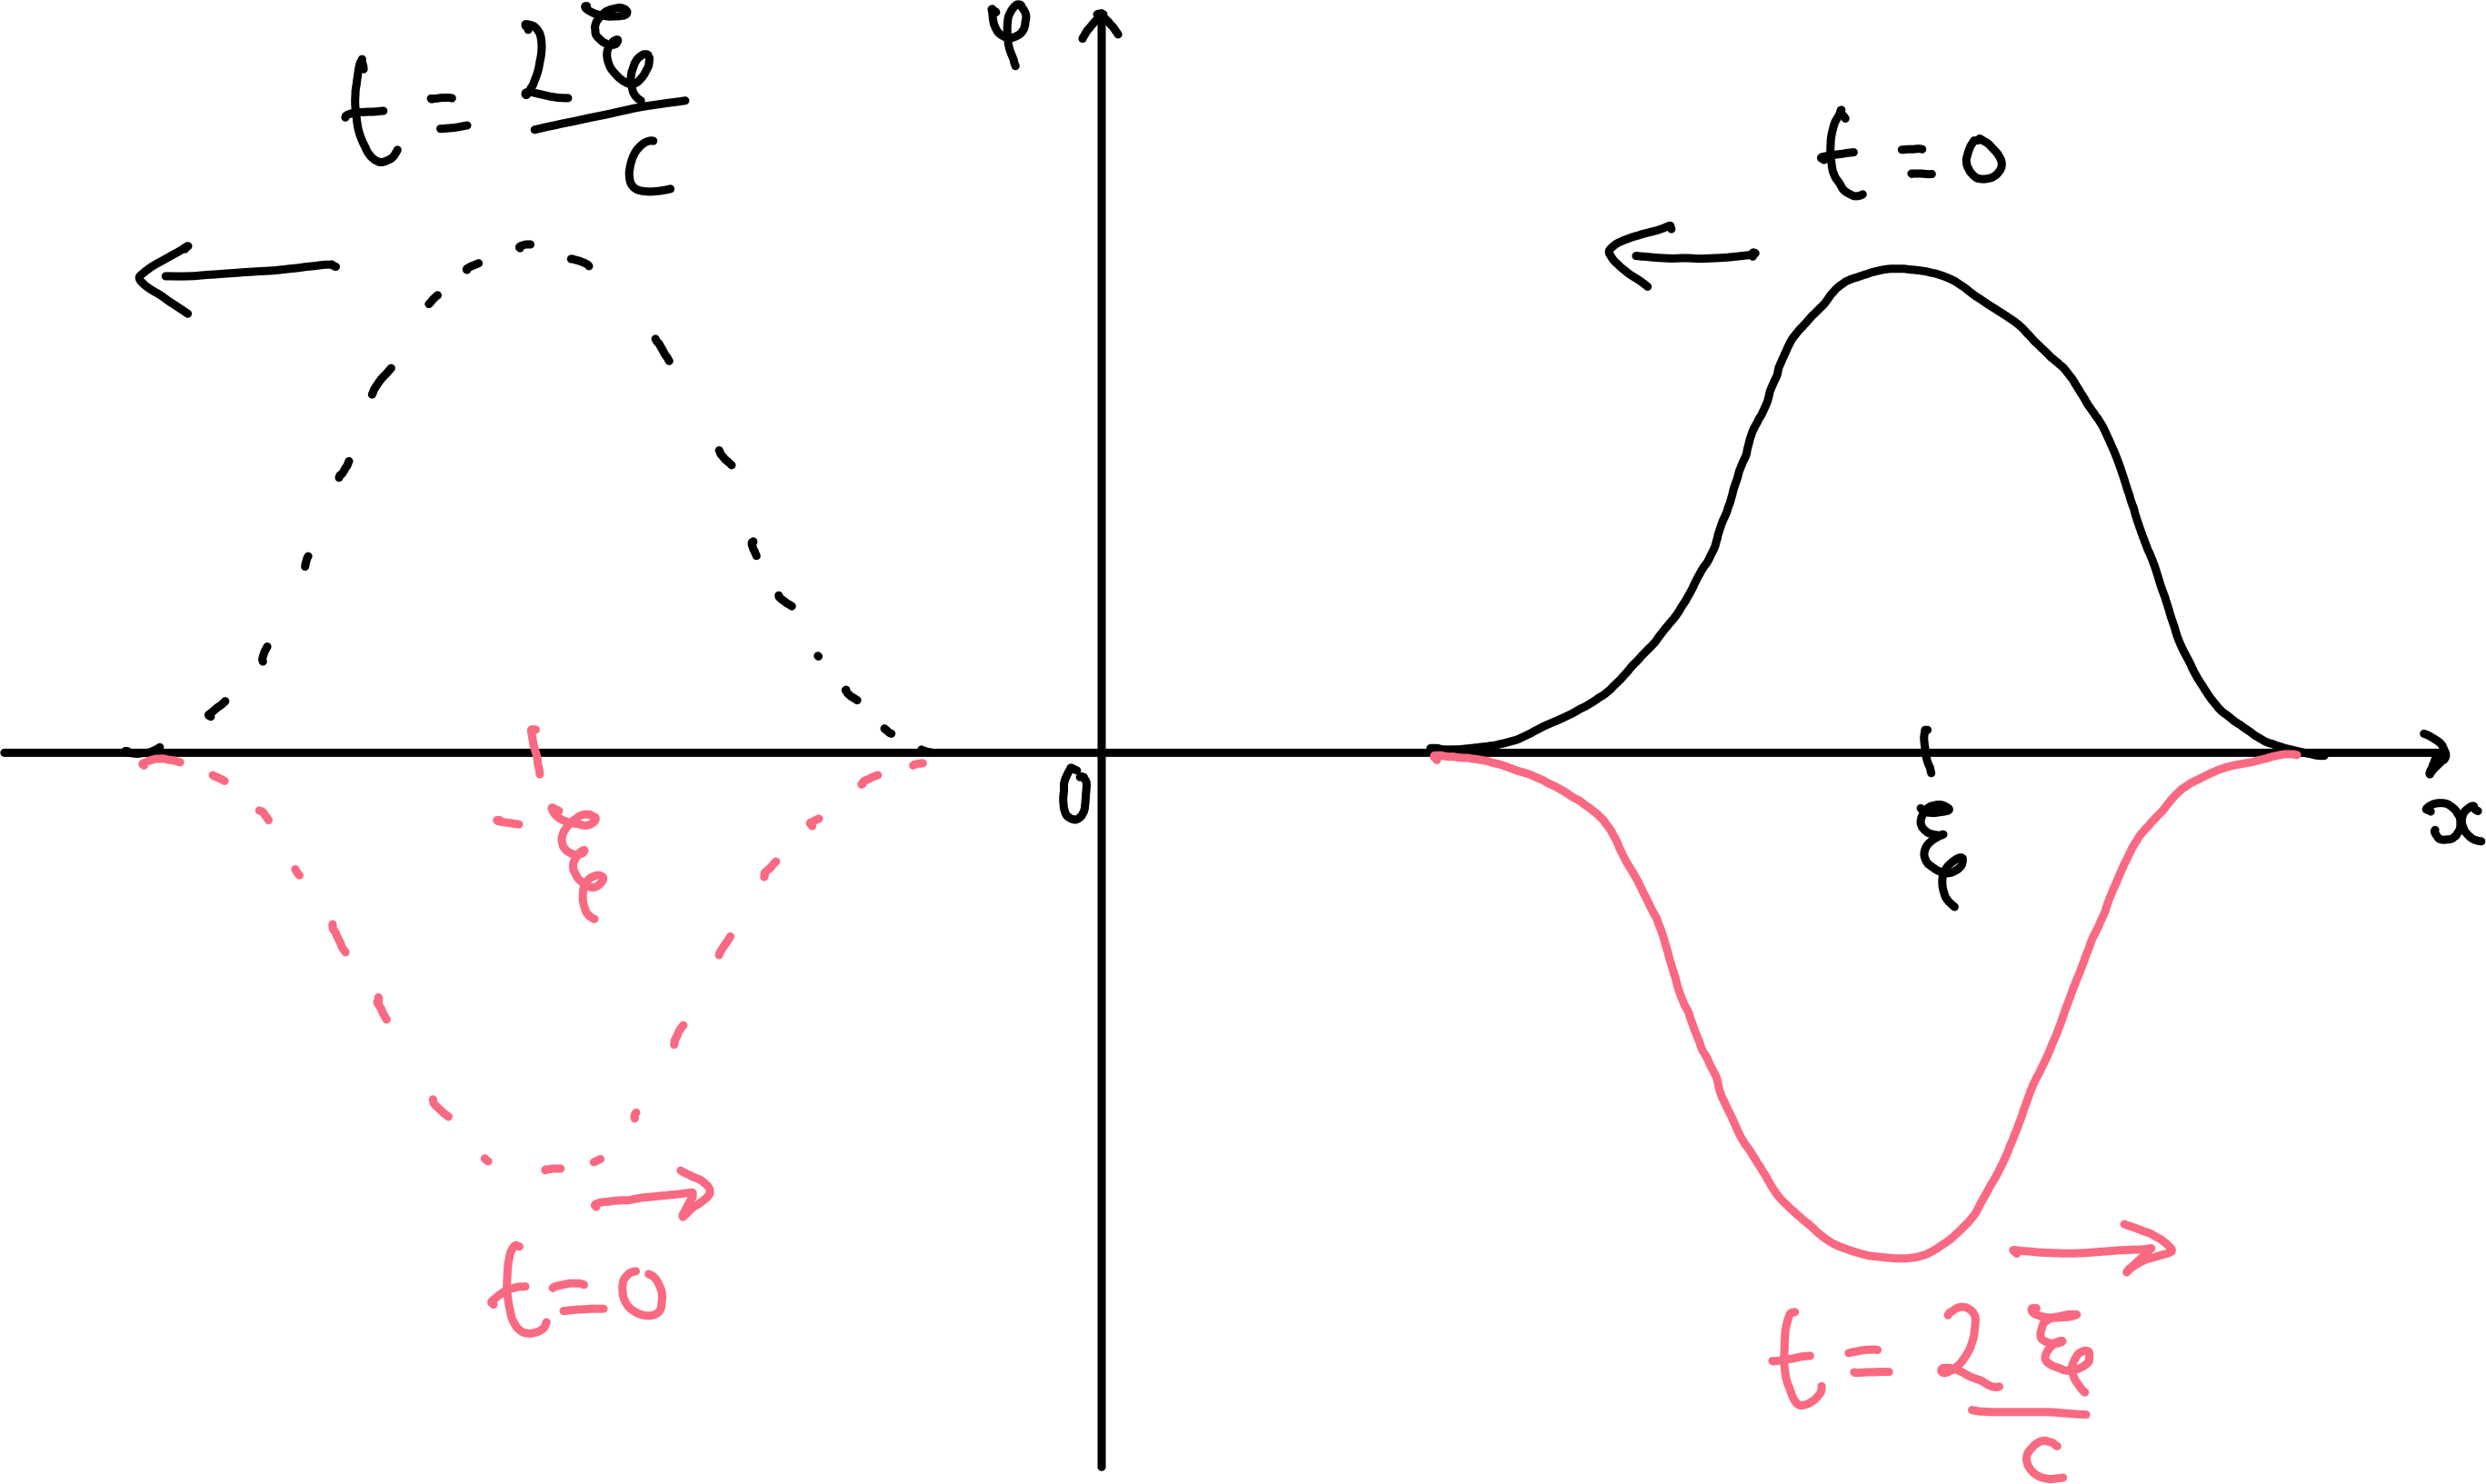
\includegraphics[height=5cm]{10-neumannImage} 
\end{figure}
The solution travels to the left, cancelling with the image at $t = \frac{\xi}{c}$, which emerges and travels right as the reflected wave.